\documentclass[a4paper,11pt, leqno]{article}
\usepackage[utf8]{inputenc}
\usepackage{graphicx}
\usepackage{fullpage}
\usepackage{indentfirst}
\usepackage[T1]{fontenc}

\title{Bubbles Commercial}
\author{Kostas Vasilopoulos}
\date{September 2018}

\begin{document}

\maketitle



\section{Introduction}

The macroeconomy and real estate markets had a good performance in 2017. Real GDP rebounded to annualized growth rates above 3.0 percent in the second and third quarters. Commercial properties in most markets enjoyed sustained growth of demand, high occupancy rates, rising rents and rising prices. These advantageous conditions may well continue into 2018, but there are several risks that might cause a change in the outlook.

\subsection{Glossary}

\textbf{REIT}
A REIT is a company dedicated to owning, and in most cases, operating income-producing real estate, such as apartments, shopping centers, offices and warehouses. Some REITs also engage in financing real estate.

\textbf{Mortgage REIT (mREIT)}
A REIT that makes or owns loans and other obligations that are secured by real estate collateral. Mortgage REITs are commonly referred to as mREITs.

\textbf{Equity REIT}
A REIT which owns, or has an "equity interest" in, rental real estate (rather than making loans secured by real estate collateral).


\subsection{Sectors}

\textbf{REITs} invest in the majority of real estate property types, including offices, apartment buildings, warehouses, retail centers, medical facilities, data centers, cell towers, infrastructure and hotels. Most REITs focus on a particular property type, but some hold multiple types of properties in their portfolios.

\textbf{Office REITs} own and manage office real estate and rent space in those properties to tenants. Those properties can range from skyscrapers to office parks. Some office REITs focus on specific types of markets, such as central business districts or suburban areas. Some emphasize specific classes of tenants, such as government agencies or biotech firms.

\textbf{Industrial REITs} own and manage industrial facilities and rent space in those properties to tenants. Some industrial REITs focus on specific types of properties, such as warehouses and distribution centers. Industrial REITs play an important part in e-commerce and are helping to meet the rapid delivery demand.

\textbf{Retail REITs} own and manage retail real estate and rent space in those properties to tenants. Retail REITs include REITs that focus on large regional malls, outlet centers, grocery-anchored shopping centers and power centers that feature big box retailers. Net lease REITs own freestanding properties and structure their leases so that tenants pay both rent and the majority of operating expenses for a property.

\textbf{Lodging REITs} own and manage hotels and resorts and rent space in those properties to guests. Lodging REITs own different classes of hotels based on features such as the hotels’ level of service and amenities. Lodging REITs’ properties service a wide spectrum of customers, from business travelers to vacationers.

\textbf{Residential REITs} own and manage various forms of residences and rent space in those properties to tenants. Residential REITs include REITs that specialize in apartment buildings, student housing, manufactured homes and single-family homes. Within those market segments, some residential REITs also focus on specific geographical markets or classes of properties.

\textbf{Timberland REITs} own and manage various types of timberland real estate. Timberland REITs specialize in harvesting and selling timber.

\textbf{Health care REITs} own and manage a variety of health care-related real estate and collect rent from tenants. Health care REITs’ property types include senior living facilities, hospitals, medical office buildings and skilled nursing facilities.

\textbf{Self-storage REITs} own and manage storage facilities and collect rent from customers. Self-storage REITs rent space to both individuals and businesses.

\textbf{Infrastructure REITs} own and manage infrastructure real estate and collect rent from tenants that occupy that real estate. Infrastructure REITs’ property types include fiber cables, wireless infrastructure, telecommunications towers and energy pipelines.

\textbf{Data center REITs} own and manage facilities that customers use to safely store data. Data center REITs offer a range of products and services to help keep servers and data safe, including providing uninterruptable power supplies, air-cooled chillers and physical security.

\textbf{Diversified REITs} own and manage a mix of property types and collect rent from tenants. For example, diversified REITs might own portfolios made up of both office and industrial properties.

\textbf{Specialty REITs} own and manage a unique mix of property types and collect rent from tenants. Specialty REITs own properties that don’t fit within the other REIT sectors. Examples of properties owned by specialty REITs include movie theaters, casinos, farmland and outdoor advertising sites.

\section{Indices}

\textbf{FTSE Nareit All REITs (FNAR)}: The FTSE Nareit All REITs Index is a market capitalization-weighted index that and includes all tax-qualified real estate investment trusts (REITs) that are listed on the New York Stock Exchange, the American Stock Exchange or the NASDAQ National Market List. The FTSE Nareit All REITs Index is not free float adjusted, and constituents are not required to meet minimum size and liquidity criteria.


\section{Analysis}


\begin{table}[!t]
\centering
\begin{tabular}{lrrr}
  \hline
 & ADF & SADF & GSADF \\ 
  \hline
Apartments & -0.18 & 3.48 & 3.56 \\ 
  Diversified & -2.10 & 1.49 & 1.98 \\ 
  FreeStanding & -0.75 & 1.66 & 2.96 \\ 
  HealthCare & -1.24 & 1.56 & 1.59 \\ 
  Industrial & -1.77 & 3.14 & 3.25 \\ 
  Lodging-Resorts & -2.25 & 2.19 & 2.19 \\ 
  ManufacturedHomes & 2.28 & 3.01 & 3.05 \\ 
  Office & -1.83 & 2.58 & 3.51 \\ 
  RegionalMalls & -1.29 & 4.94 & 4.96 \\ 
  Residential & 0.08 & 3.29 & 3.35 \\ 
  Retail & -1.44 & 4.15 & 4.43 \\ 
  SelfStorage & 1.01 & 4.46 & 4.46 \\ 
  ShoppingCenters & -1.84 & 3.52 & 4.03 \\ 
  ----- &  &  &  \\ 
  Crit Values &  &  &  \\ 
  90\% & -0.44 & 1.11 & 1.87 \\ 
  95\% & -0.12 & 1.44 & 2.18 \\ 
  99\% & 0.66 & 2.01 & 2.70 \\ 
   \hline
\end{tabular}
\end{table}

\begin{figure}
    \centering
    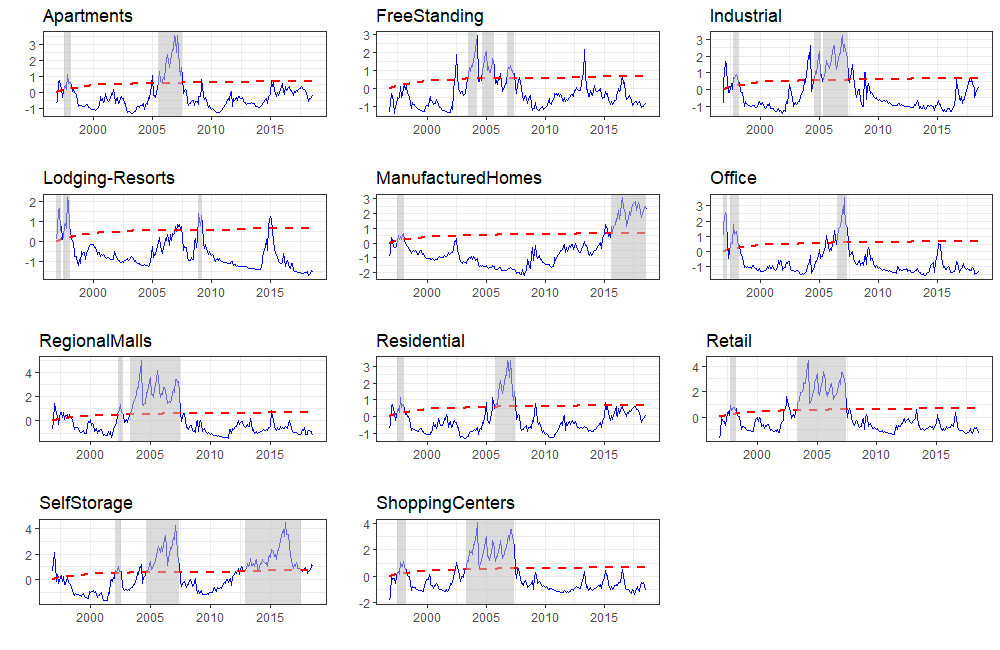
\includegraphics[scale = 0.6]{individual.png}
    \caption{Caption}
    \label{fig:my_label}
\end{figure}

\begin{figure}
    \centering
    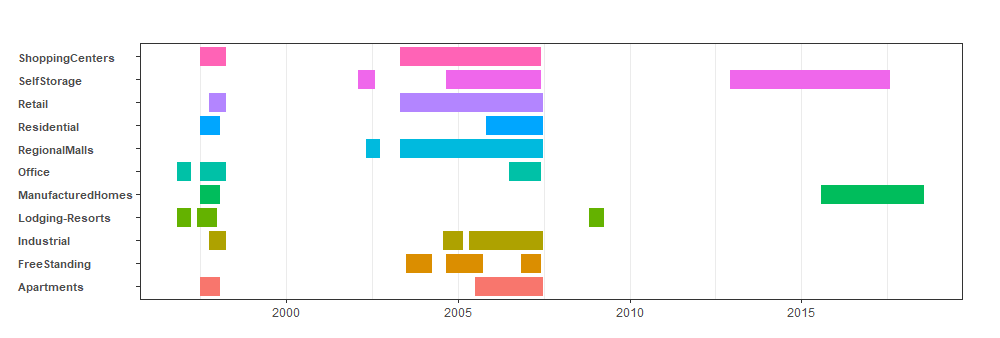
\includegraphics[scale = 0.65]{datestamp.png}
    \caption{Caption}
    \label{fig:my_label}
\end{figure}



\end{document}
